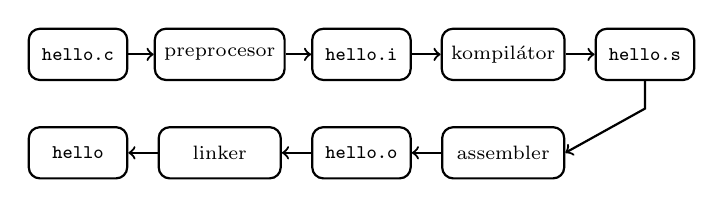
\begin{tikzpicture}[
    file/.style={
        draw,
        rounded corners,
        thick,
        align=center,
        font=\scriptsize,
        minimum width=1.25cm,
        minimum height=0.65cm
    },
    tool/.style={
        draw,
        rounded corners,
        thick,
        align=center,
        font=\scriptsize,
        minimum width=1.55cm,
        minimum height=0.65cm
    },
    arrow/.style={->, thick}
]

    \node<3->[file] (c) at (0,0) {\texttt{hello.c}};
    \node<3->[tool] (pre) at (1.8,0) {preprocesor};
    \node<3->[file] (i) at (3.6,0) {\texttt{hello.i}};

    \draw<3->[arrow] (c) -- (pre);
    \draw<3->[arrow] (pre) -- (i);

    \node<4->[tool] (comp) at (5.4,0) {kompilátor};
    \node<4->[file] (s) at (7.2,0) {\texttt{hello.s}};

    \draw<4->[arrow] (i) -- (comp);
    \draw<4->[arrow] (comp) -- (s);

    \node<5->[tool] (asm) at (5.4,-1.25) {assembler};
    \node<5->[file] (o) at (3.6,-1.25) {\texttt{hello.o}};

    \draw<5->[arrow] (s.south) -- ++(0,-0.35) -- (asm.east);
    \draw<5->[arrow] (asm) -- (o);

    \node<6->[tool] (link) at (1.8,-1.25) {linker};
    \node<6->[file] (exe) at (0,-1.25) {\texttt{hello}};

    \draw<6->[arrow] (o) -- (link);
    \draw<6->[arrow] (link) -- (exe);

\end{tikzpicture}
